\documentclass[dvipsnames,tikz]{standalone}
\usepackage{amsmath}
\usepackage{arevmath}
\usepackage{xcolor}
\usepackage{tikz}
\usetikzlibrary{calc}
\usetikzlibrary{decorations.pathreplacing,calligraphy,3d}
\usetikzlibrary{lindenmayersystems}
\usepackage{pgfplots}
\pgfplotsset{compat = newest}

\tikzset{main/.style={draw=black, color=black}}


\begin{document}
	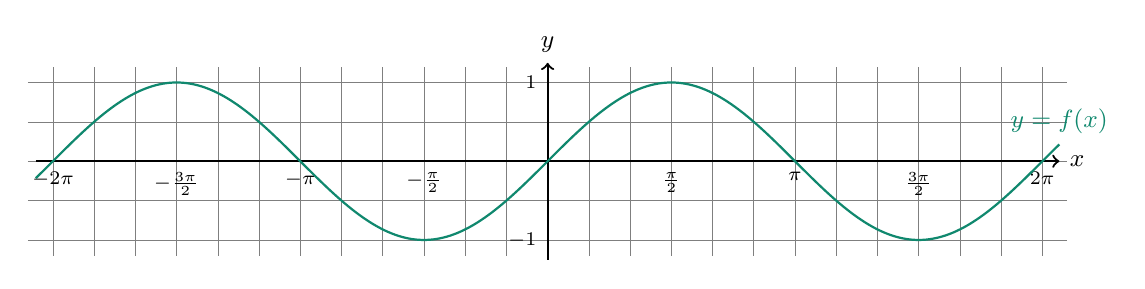
\begin{tikzpicture}[font=\small, tl/.style = {black, inner sep=1pt, font=\scriptsize} ]
		% grid
		\draw[main, very thin, xstep=0.5235, ystep=0.5, semitransparent] (-6.6,-1.2) grid (6.6,1.2);
		
		% y tick label
		\foreach \y in {-1, 1}{\node[tl,left=1mm] at (0,\y) {$\y$};}
		% x tick label
		\foreach \x [count=\xx from -4] in 
		{-2\pi,          %-\frac{11\pi}{2}, -\frac{5\pi}{3},
			-\frac{3\pi}{2},%-\frac{4\pi}{3},  -\frac{7\pi}{6},
			-\pi,           %-\frac{5\pi}{6},  -\frac{2\pi}{3},
			-\frac{\pi}{2}, %-\frac{4\pi}{3},  -\frac{7\pi}{6},
			{ },
			%\frac{\pi}{6},  \frac{\pi}{3},   
			\frac{\pi}{2},
			%\frac{2\pi}{3}, \frac{5\pi}{6},
			\pi,           %-\frac{7\pi}{6},   \frac{4\pi}{3},
			\frac{3\pi}{2}, %-\frac{5\pi}{3},  \frac{11\pi}{6},
			2\pi
		}{\node[tl,below=1mm] at (3*0.5235*\xx,0) {$\x$};}
		% axes
		\draw[main, ->,thick] (-6.5,0) -- (6.5,0) node[right] {$x$};
		\draw[main, ->,thick] (0,-1.25) -- (0, 1.25) node[above] {$y$};
		% curve
		\draw[thick,PineGreen, draw=PineGreen,	domain=-6.5:6.5,samples=300,variable=\x] plot(\x,{sin(deg{\x})}) node [above] {$y=f(x)$};
	\end{tikzpicture}
\end{document}